\subsection{The variational principle}

\begin{frame}[label=variationalprinc]{The variational principle}
  \vspace{-10pt}
  \begin{itemize}[<+->]
    \item Name derived from calculus of variations which deals with maximising or minimising functionals.
    \begin{table}
      \begin{tabular}{l  l  l }
      Functions   &$p:\theta \mapsto \bbR$  &(standard calculus) \\ 
      Functionals &$\cH:p \mapsto \bbR$     &(variational calculus) \\ 
      \end{tabular}
    \end{table}
  \item Using standard calculus, we can solve
  \[
    \argmax_\theta p(\theta) =: \hat\theta
  \]
  e.g. $p$ is a likelihood function, and $\hat\theta$ is the ML estimate.
  \item Using variational calculus, we can solve
  \[
    \argmax_p \cH(p) =: \tilde p
  \]
  e.g. $\cH$ is the entropy $\cH = - \int p(x)\log p(x) \d x$, and $\tilde p$ is the entropy maximising distribution.
  \end{itemize}
  \vspace{5pt}
  
  \begin{textblock*}{3cm}(.982\textwidth,1.04\textheight)%
    \hyperlink{idea}{\beamerbutton{back}}      
  \end{textblock*}
\end{frame}

\subsection{Comparison to EM}

\subsection{The EM algorithm}
\begin{frame}[label=emalg]{Comparison to the EM algorithm }
  \begin{itemize}
    \setlength\itemsep{0.5em}
    \item In addition to latent variables $\bz$, typically there are unknown parameters $\theta$ to be estimated.
    \begin{itemize}
      \item Frequentist estimation: $\theta$ is fixed
      \item Bayesian estimation: $\theta \sim p(\theta)$ is random
    \end{itemize}
    \item Consider $\theta$ fixed. Maximising the (marginal) log-likelihood directly
      \begin{align*}
        \argmax_\theta \ \log \bigg\{\int \myoverbrace{p(\by|\bz,\theta)p(\bz|\theta)}{p(\by,\bz)} \d\bz \bigg\}
      \end{align*}
    is difficult. However, if somehow the latent variables were known, then the problem may become easier.
    \item Given initial values $\theta^{(0)}$, the EM algorithm cycles through\vspace{0.2em}
        \begin{itemize}\setlength\itemsep{0.2em}
          \item \textbf{E-step}: Compute $Q(\theta|\theta^{(t)}) := \E_\bz[\log p(\by,\bz|\theta) \,|\, \by,\theta^{(t)}] $ \vspace{0.3em}
          \item \textbf{M-step}: $\theta^{(t+1)} \gets \argmax_\theta Q(\theta|\theta^{(t)})$
        \end{itemize}
        for $t=1,2,\dots$ until convergence.
  \end{itemize}

\end{frame}

\begin{frame}{Comparison to the EM algorithm (cont.)}
    \onslide<1->{
  {\footnotesize\renewcommand{\arraystretch}{1.5}
  \begin{table}[]
  \centering
  \begin{tabular}{p{5cm}p{5cm}}
  \toprule
  Variational inference/Bayes & (Variational) \hyperlink{emalg}{EM algorithm}\\ 
  \midrule
  \textbf{GOAL}: Posterior densities for $(\bw, \theta)$                                                          
  & \textbf{GOAL}: ML/MAP estimates for $\theta$ \\
  Variational approximation for latent variables and parameters $q(\bw,\theta)\approx p(\bw,\theta|\by)$ 
  & Variational approximation for latent variables only $q(\bw)\approx p(\bw|\by)$ \\
  Priors required on $\theta$                                                                            
  & Priors not necessary for $\theta$ \\
  Derivation can be tedious 
  & Derivation less tedious \\
  Inference on $\theta$ through (approximate) posterior density $q(\theta)$
  & Asymptotic distribution of $\theta$ not well studied; standard errors for $\theta$ not easily obtained \\
  \bottomrule
  \end{tabular}
  \end{table}
  }}
  
  \begin{textblock*}{3cm}(.982\textwidth,1.04\textheight)%
    \hyperlink{compareemalg}{\beamerbutton{back}}      
  \end{textblock*}
\end{frame}

\subsection{Laplace's method}

\begin{frame}[label=laplace]{Laplace's method}
  \blfootnote{\fullcite[§4.1, pp.777-778.]{Kass1995}}
  \vspace{-15pt}
  \begin{itemize}[<+->]\setlength\itemsep{0.8em}
    \item Interested in $p(\bff|\by) \propto p(\by|\bff)p(\bff) =: e^{Q(\bff)}$, with normalising constant $p(\by) = \int e^{Q(\bff)} \d\bff$. The Taylor expansion of $Q$ about its mode $\tilde\bff$
    \[
      Q(\bff) \approx Q(\tilde\bff) - \half (\bff - \tilde\bff)^\top\bA(\bff - \tilde\bff) 
    \]
    is recognised as the logarithm of an unnormalised Gaussian density, with $\bA = -\text{D}^2 Q(\bff)$ being the negative Hessian of $Q$ evaluated at  $\tilde\bff$.
    \item The posterior $p(\bff|\by)$ is approximated by $\N(\tilde\bff, \bA^{-1})$, and the marginal by
    \[
      p(\by) \approx (2\pi)^{n/2} \vert \bA \vert^{-1/2}  p(\by|\tilde\bff)p(\tilde\bff)
    \]
    \item Won't scale with large $n$; difficult to find modes in high dimensions.
  \end{itemize}
  
  \begin{textblock*}{3cm}(.982\textwidth,1.04\textheight)%
    \hyperlink{quality}{\beamerbutton{back}}      
  \end{textblock*}
\end{frame}

\begin{frame}[label=varcompare]{Comparison of approximations (density)}
  \vspace{-5pt}
  \only<1|handout:0>{
    \begin{center}
      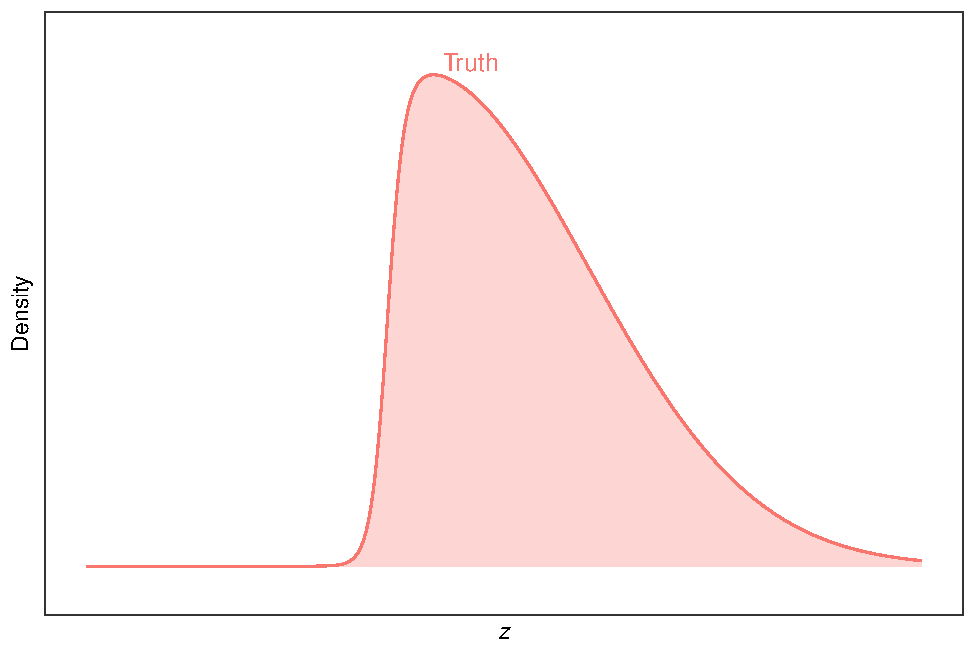
\includegraphics[scale=0.7]{figure/compare1}
    \end{center}
  }
%  \only<2|handout:0>{
%    \begin{center}
%      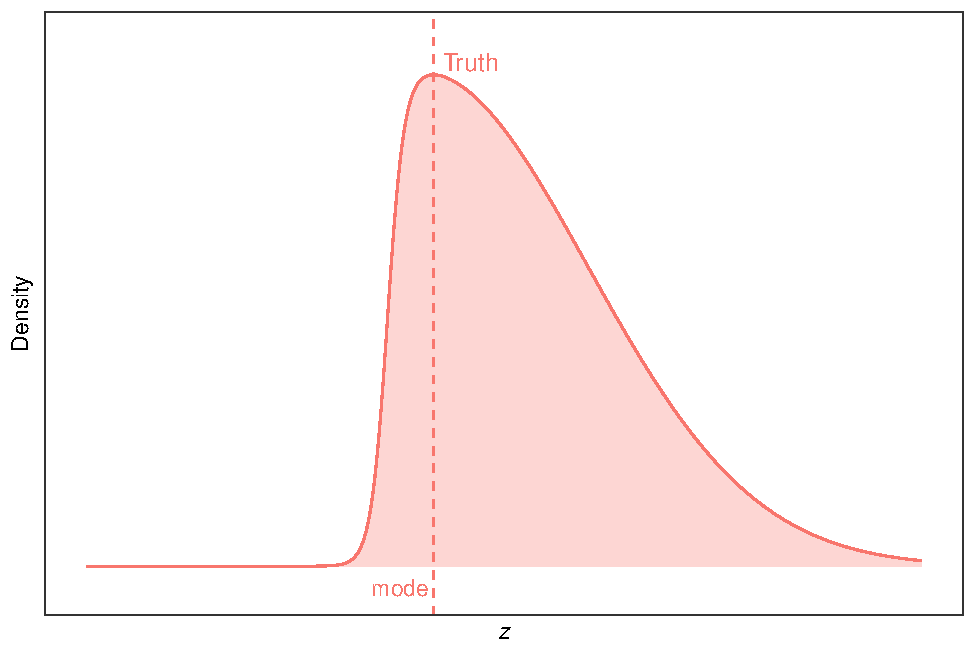
\includegraphics[scale=0.7]{figure/compare2}
%    \end{center}
%  }  
  \only<2|handout:0>{
    \begin{center}
      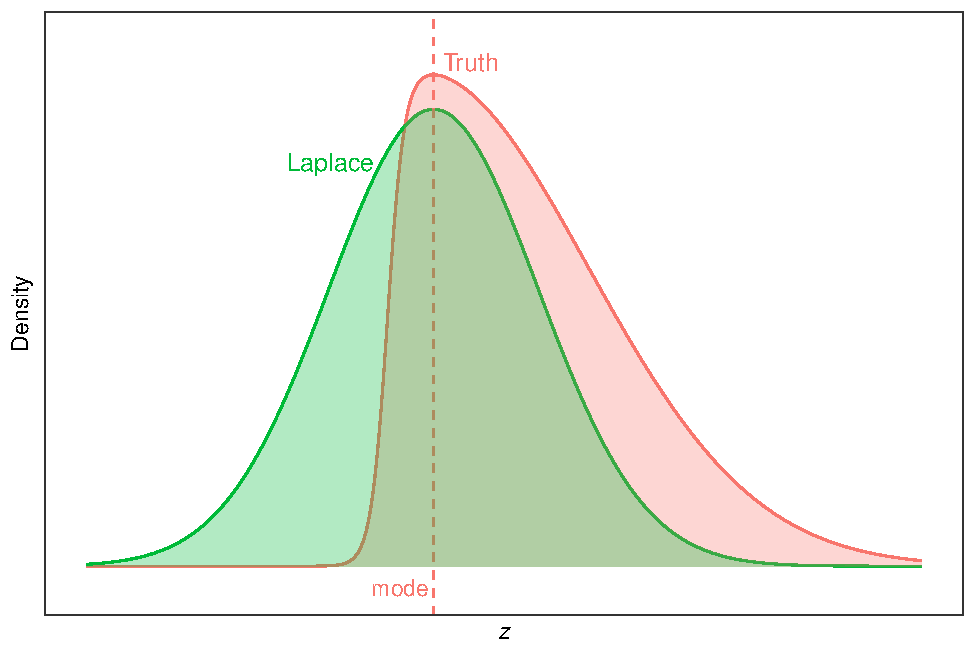
\includegraphics[scale=0.7]{figure/compare3}
    \end{center}
  } 
%  \only<4|handout:0>{
%    \begin{center}
%      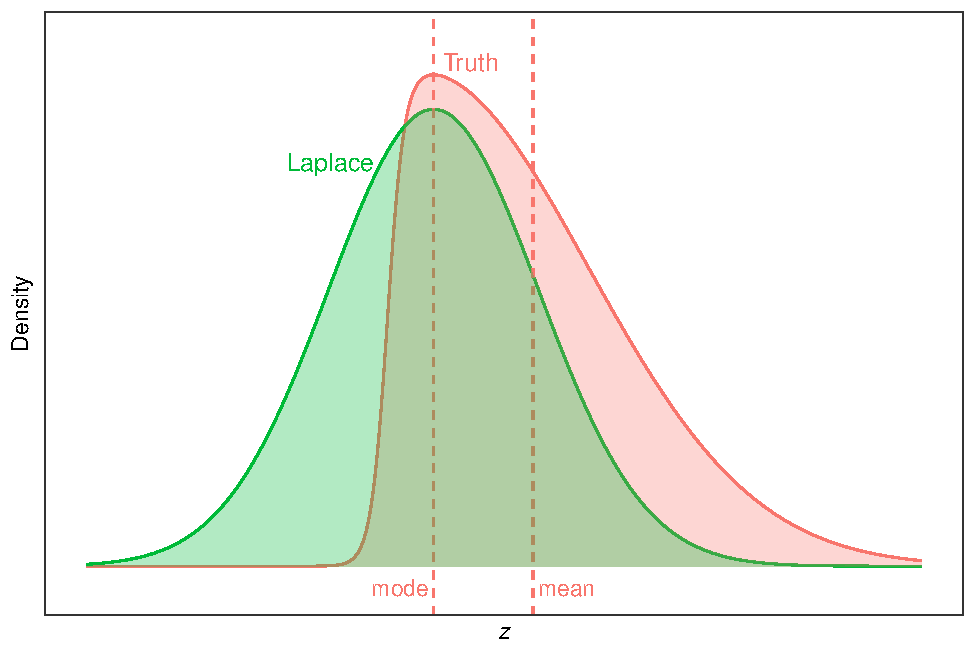
\includegraphics[scale=0.7]{figure/compare4}
%    \end{center}
%  } 
  \only<3|handout:1>{
    \begin{center}
      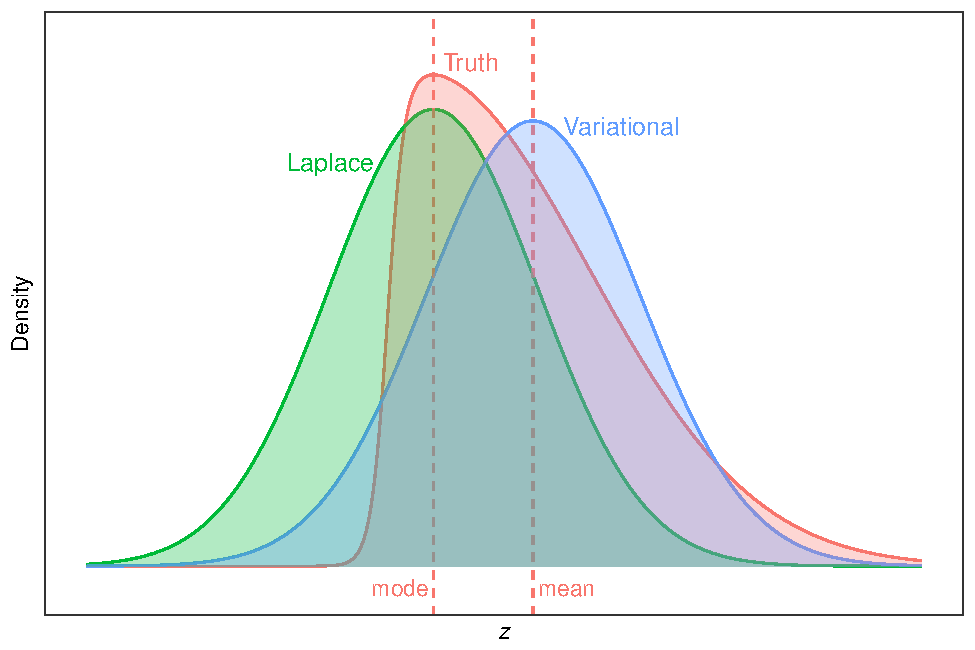
\includegraphics[scale=0.7]{figure/compare5}
    \end{center}
  } 
  
  \begin{textblock*}{3cm}(.982\textwidth,1.04\textheight)%
    \hyperlink{quality}{\beamerbutton{back}}      
  \end{textblock*}
\end{frame}

\begin{frame}{Comparison of approximations (deviance)}
  \vspace{-5pt}
  \begin{center}
    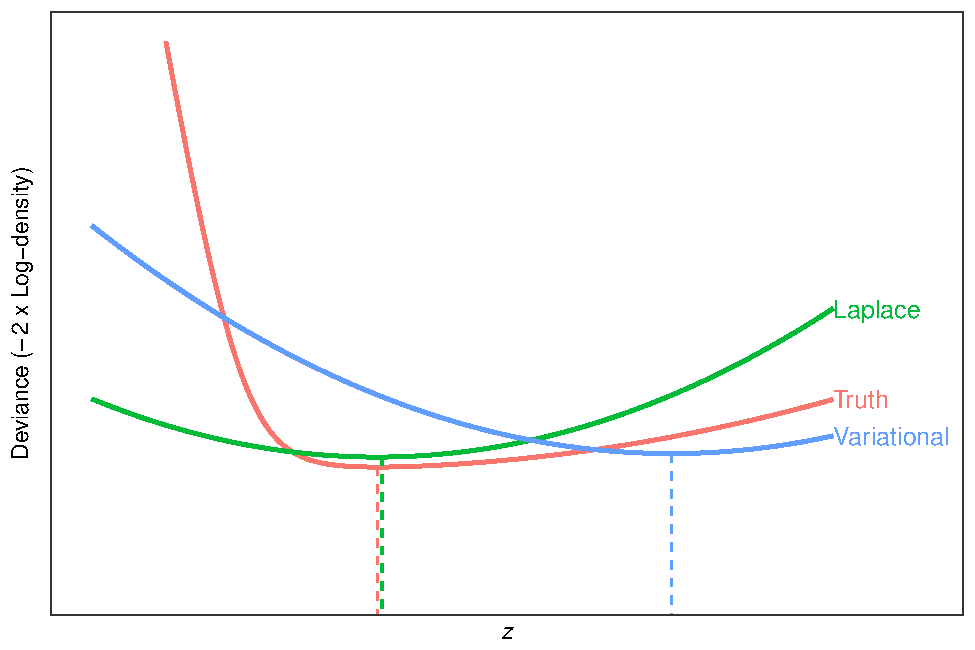
\includegraphics[scale=0.7]{figure/compare6}
  \end{center}

  \begin{textblock*}{3cm}(.982\textwidth,1.04\textheight)%
    \hyperlink{quality}{\beamerbutton{back}}      
  \end{textblock*}  
\end{frame}

\subsection{Solutions to Gaussian mixture}

\begin{frame}[label=vigmmsoln]{Variational solutions to Gaussian mixture model}
  \underline{Variational M-step}
  \begin{align*}
  \begin{gathered}
    \tilde q(\bz) = \prod_{i=1}^n\prod_{k=1}^K r_{ik}^{z_{ik}}, \hspace{0.5cm} r_{ik} = \rho_{ik} / \sum_{k=1}^K \rho_{ik} \\
    \log \rho_{ik} = \E[\log\pi_k] + \half \E\big[\log|\bPsi_k|\big] - \half[d]\log 2\pi \\
    - \half \E \left[(\bx_i - \bmu_k)^\top \bPsi_k (\bx_i - \bmu_k)  \right]
  \end{gathered} 
  \end{align*}
  \underline{Variational E-step}
  \begin{align*}
  \begin{gathered}
    \tilde q(\pi_1,\dots,\pi_K) = \Dir_K(\bpi | \tilde\balpha),  \hspace{0.5cm}  \tilde\alpha_k = \alpha_{0k} + \textstyle\sum_{i=1}^n r_{ik} \\
    \tilde q(\bmu,\bPsi) = \prod_{k=1}^K \N_d\big(\bmu_k|\tilde\bmm_k, (\tilde\kappa_{k}\bPsi_k)^{-1}\big)\Wis_d(\bPsi_k|\tilde\bW_k,\tilde\nu_k)
  \end{gathered} 
  \end{align*}
  
  \begin{textblock*}{3cm}(.982\textwidth,1.04\textheight)%
    \hyperlink{vigmm}{\beamerbutton{back}}      
  \end{textblock*} 
\end{frame}

\begin{frame}{Variational solutions to Gaussian mixture model (cont.)}
  \vspace{-20pt}
  \begin{align*}
  \begin{gathered}
    \tilde\kappa_k = \kappa_0 + \textstyle\sum_{i=1}^n r_{ik} \\
    \tilde\bmm_k = (\kappa_0\bmm_0 + \textstyle\sum_{i=1}^n r_{ik}\bx_i) / \tilde\kappa_k \\
    \bW_k^{-1} = \bW_0^{-1} + \sum_{i=1}^n r_{ik}(\bx_i - \bar\bx_k)(\bx_i - \bar\bx_k)^\top \\
    \bar\bx_k = \sum_{i=1}^n r_{ik}\bx_i \Big/ \sum_{i=1}^n r_{ik} \\
    \nu_k = \nu_0 + \textstyle\sum_{i=1}^n r_{ik}
  \end{gathered} 
  \end{align*}
  \underline{Also useful}
  \begin{align*}
  \begin{gathered}
    \E \left[(\bx_i - \bmu_k)^\top \bPsi_k (\bx_i - \bmu_k)  \right] = 
    d/\tilde\kappa_k + \nu_k(\bx_i - \tilde\bmm_k)^\top \tilde\bW_k (\bx_i - \tilde\bmm_k) \\
    \E[\log\pi_k] = \textstyle\sum_{i=1}^d \psi\left(\frac{\nu_k + 1 - i}{2} \right) + d \log 2 + \log |\tilde\bW_k |  \\
    \E\big[\log|\bPsi_k|\big] = \psi(\tilde\alpha_k) - \psi\big(\textstyle\sum_{k=1}^K\tilde\alpha_k\big), \hspace{0.5cm} \psi(\cdot)\text{ is the digamma function}
  \end{gathered} 
  \end{align*}  
  
  \begin{textblock*}{3cm}(.982\textwidth,1.04\textheight)%
    \hyperlink{vigmm}{\beamerbutton{back}}      
  \end{textblock*} 
\end{frame}
